\documentclass{article}
\usepackage[utf8]{inputenc}
\usepackage[ngerman]{babel}

\title{Einführung Simulation PS-Aufgabe 2021:\\Notaufnahme}
\author{Sofia Bonini, Dario Leon Hornsteiner, Sabine Daniela Hasenleithner}
\date{\today}

\usepackage{natbib}
\usepackage{graphicx}

\begin{document}

\maketitle

\section{Anforderungen an das Simulationsprojekt mit integrierten Erweiterungen}
Die Aufgabe war es eine Notaufnahme eines Krankenhauses zu simulieren. In der Notaufnahme des Krankenhauses erscheint durchschnittlich alle 40 Minuten ein Patient, wobei tagsüber immer zwei Ärzte und nachts ein Arzt im Einsatz sind. Jeder Patient muss eine Erst- und eine Zweit-Behandlung durchleben, bevor er das Krankenhaus verlässt. Ein Ausnahmefall besteht, wenn der Patient ein Notfallpatient ist und die Wartezeit in der Schlange so lange andauert, dass er noch in der Warteschlange verstirbt.\\
Etwa 20\% der Patienten müssen möglichst rasch behandelt werden und werden als akute Notfälle eingestuft, der Rest wird als regulärer Patient in die Warteschlange eingelassen und kann länger warten. Es gibt noch eine dritte Kategorie der Patienten, die die Covid-19-Verdachtsfälle darstellen (ca. 5\%). Bevor die Patienten das Krankenhaus betreten, wird durch eine Fiebermessstation überprüft, ob es sich um einen Covid-Verdachtsfall handelt, wenn ja wird dieser umgehend zu einer gesonderten Warteschlange weitergeleitet, um die sich ein eigener Arzt kümmert und immer 10 Minuten zwischen den Behandlungen die Station desinfiziert.\\
Den akuten Notfällen wird die Priorität 3 zugeordnet, dann Reduktion der Priorität auf 2. Hier warten die Patienten nun bis wieder ein Arzt verfügbar ist, um nochmals behandelt zu werden, vor Verlassen der Notaufnahme. Jenen Patienten, die warten können wird Priorität 1 zugeordnet und erhalten dann ebenfalls Priorität 2, zur Zweitbehandlung, danach verlassen auch diese die Notaufnahme.\\
\\
Das Experiment simuliert 20 Tage, denen 2 Tage Initialisierung (Warm-UP Phase) davor angehängt werden. Somit werden insgesamt 22 Tage simuliert. Zusätzlich werden 50 sogenannter 'Runs' durchgeführt, um ein möglichst akkurates Ergebnis zu erhalten.\\


\subsection{Zu ermittelnde Werte}
\begin{itemize}
    \item jeweils maximale und mittlere Anzahl der wartenden akuten Notfälle und restlichen Patienten
    \item die mittlere Wartezeit beider Patientenarten
    \item Anteil jener Patienten, die nicht warten müssen
    \item Anteil der Patienten, welche maximal 5 Minuten warten müssen
    \item jene Zeit x, sodass 90\% der Patienten maximal x Zeiteinheiten in der Notaufnahme verbringen (vom Eintreffen bis zum Verlassen nach Behandlungsende) - genannt 90\%-Quantile
    \item Anzahl der Notfall-Patienten. die bereits in der Warteschlange sterben
    \item Ankunftszeiten des Tag/ Nacht Zyklus
\end{itemize}

\section{Implementierung}

Es wurde ein prozessorientierter Ansatz in der Implementierung verfolgt, da so die Abbildung aktiver und passiver Phasen von Komponenten näher an der Realität sind, also besser darstellbar sind. Die jeweiligen Komponenten wurden deshalb in Unterklassen der von DESMO-J zur Verfügung gestellten abstrakten Klasse \texttt{SimProcess} umgesetzt.

Die Implementierung umfasst folgende Klassen:

\subsection{PatientProcess}
Dem Konstruktor der Klasse \texttt{PatientProcess} werden zwei Booleans übergeben,
die definieren, ob der entsprechende Patient ein Notfall-Patient ist und ob er ein COVID-Verdachtsfall ist.

Der Lebenszyklus eines Patienten beginnt mit dem Betreten der Notaufnahme.
In der Praxis wird hier die Körpertemparatur gemessen und bei erhöhter Temparatur wird der Patient als COVID-Verdachtsfall eingestuft.
In der Simulation gilt einfach ein gewisser Prozentsatz der Patienten (5\%) als COVID-Verdachtsfall.
Um COVID-Verdachtsfälle zu isolieren, wird eine separate Station simuliert (durch eigene Warteschlange und Personal, siehe \textit{CovidDocProcess}).
Um die Ansteckungsgefahr im Warteraum weiter zu reduzieren,
wird bei COVID-Verdachtsfällen die Erst- und Zweitbehandlung direkt im Anschluss aneinander durchgeführt.

Für Patienten ohne erhöhte Temperatur gibt es beim Betreten der Notaufnahme zwei Möglichkeiten:
Wenn gerade ein Arzt verfügbar ist, kann der Patient direkt behandelt werden.
Ansonsten muss er warten.
Dies wird in der Simulation allerdings so umgesetzt,
dass der Patient in jedem Fall in die entsprechende Warteschlange
(für Notfall- oder normale Patienten) eingefügt wird,
und wenn ein Arzt verfügbar ist, dieser den Patienten sofort wieder herausnimmt.
Um herauszufinden, ob ein Arzt verfügbar ist, verwendet der Patient die Methode \texttt{findDoc()},
in der ein Arzt, wenn verfügbar,
aus der Ärzte-Warteschlange des \texttt{EmergencyModel} herausgenommen wird und im Anschluss aktiviert werden kann.

Nach der Erstbehandlung wiederholt sich dieser Prozess, indem der Patient in eine eigene Warteschlange für Zweitbehandlungen eingereiht wird (Priorität zwischen Notfällen und normalen Erstbehandlungen) und je nach Verfügbarkeit eines Arztes noch einmal auf seine Behandlung warten muss. Nach der Zweitbehandlung verlässt der Patient die Notaufnahme.\\

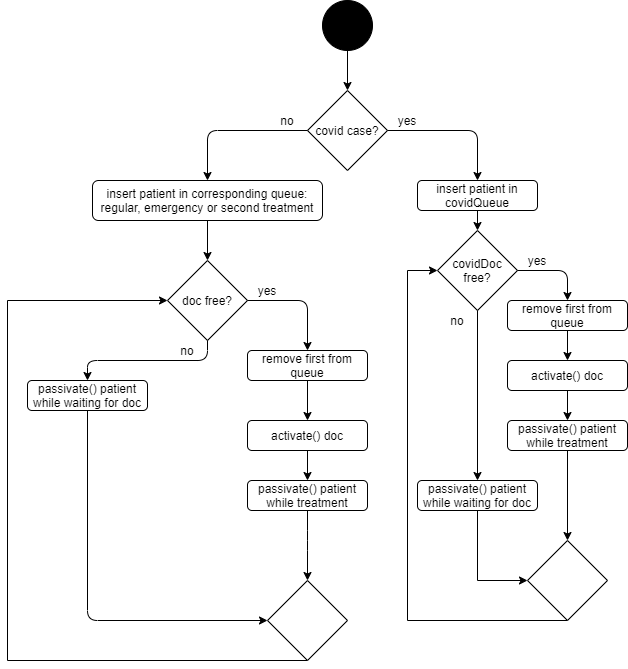
\includegraphics[width=\textwidth]{img/patientProcess.png}
\textit{Vereinfachte Version des 'LifeCycle' des PatientProcess}

\subsection{NewPatientProcess}

Die Klasse \texttt{NewPatientProcess} stellt eine Hilfsklasse dar, die in wiederkehrenden Abständen neue Patienten generiert. Dazu wird der Prozess in einer Schleife für eine zufällige Zeit angehalten, die durch \\ \texttt{EmergencyModel.getPatientArrivalTime()} bestimmt wird. Im Anschluss wird ein neuer Prozess der Klasse \texttt{PatientProcess} erzeugt und aktiviert. 

Dazu wird im \texttt{EmergencyModel} ein Wert aus der Exponentialverteilung \\ \texttt{avgArrivalTime} um den Durchschnittswert von 40 Minuten gezogen, wobei negative Werte ausgeschlossen sind.

Um festzulegen, ob der erzeugte Patient COVID-Verdachtsfall und Notfallpatient ist, werden \texttt{EmergencyModel.hasCovid()} und \\ \texttt{EmergencyModel.isEmergency()} verwendet. Dabei werden jeweils Werte aus Gleichverteilungen zwischen 0 und 1 gezogen und mit einem Schwellwert verglichen (0.05 für COVID, 0.2 für Notfälle), sodass durchschnittlich 5\% aller Patienten COVID-Verdachtsfälle und 20\% Notfälle sind.

\begin{center}
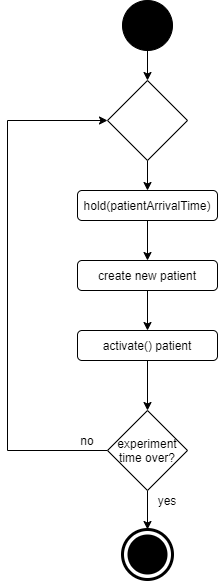
\includegraphics[scale=0.55]{img/newPatientProcess.png} \\
\textit{Vereinfachte Version des 'LifeCycle' des NewPatientProcess}
\end{center}

\subsection{DocProcess}

Die Priorisierung der Patienten wurde zunächst mithilfe von \\ \texttt{SimProcess.setSchedulingPriority()} und der \texttt{ProcessQueue} umgesetzt, die diese Priorität berücksichtigt.
Um eine detailliertere statistische Auswertung zu erlauben, wurden jedoch später separate Warteschlangen für Notfälle, Erst- und Zweitbehandlung eingeführt.
Es liegt daher nun in der Verantwortung des \texttt{DocProcess}, die Prioritäten zu beachten.
Daher überprüft ein Arzt immer zuerst die Warteschlange der Notfälle, dann die der Zweitbehandlungen und schließlich die der Nicht-Notfälle.

Sobald eine Warteschlange besetzt ist, entfernt der Arzt den jeweiligen Patienten aus der Warteschlange und beginnt die Behandlung.
Dazu wird \\ \texttt{EmergencyModel.getTreatmentTime()} aufgerufen und der Arzt für die entsprechende Zeitspanne durch \texttt{hold()} in einen passiven Zustand versetzt.
Der Methode werden dabei Parameter übergeben, die aussagen, ob es sich um einen Notfallpatienten und um eine Erstbehandlung handelt.
Mithilfe verschiedener Gleichverteilungen wird dann eine entsprechende Behandlungszeit gezogen.
Notfallpatienten haben dabei durchschnittlich eine doppelt so lange Behandlungszeit wie andere Patienten:\\

\begin{tabular}{ccc}
Zeit in Minuten & \textbf{normale Behandlung} & \textbf{Notfall-Behandlung} \\
\textbf{Erstbehandlung} & 15 - 60 & 30 - 120 \\
\textbf{Zweitbehandlung} & 5 - 30  & 10 -  60
\end{tabular}
\\\\

Der Arzt versetzt sich selbst für die Behandlungszeit in einen passiven Zustand und aktiviert im Anschluss den \texttt{PatientProcess}, damit dieser sich entweder für die Zweitbehandlung einreiht oder die Notaufnahme verlässt.

Für den Fall, dass in keiner der Warteschlangen Patienten warten,
fügt sich der jeweilige Arzt selbst in die Ärzte-Warteschlange des \texttt{EmergencyModel} ein und versetzt sich in einen passiven Zustand,
bis er wieder von einem Patienten aktiviert wird.

\subsection{CovidDocProcess}

Der COVID-Arzt ist nur dafür zuständig, Verdachtsfälle zu behandeln.
Da sich der Lebenszyklus des Arztes auf der COVID-Station so stark von den anderen Ärzten unterscheidet,
wurde er in einen eigenen Prozess ausgelagert.
Die Unterschiede sind, dass der Arzt lediglich die Warteschlange für COVID-Patienten überprüft, bevor er Behandlungen beginnt; und dass er nach jeder Behandlung zusätzlich 10 Minuten Zeit benötigt, um die Station zu desinfizieren.

Die Behandlungszeit für COVID-Patienten beträgt 15-60 Minuten (für sie gibt es keine Zweitbehandlung).

Im \texttt{EmergencyModel} gibt es eine eigene Warteschlange für den Covid-Arzt.

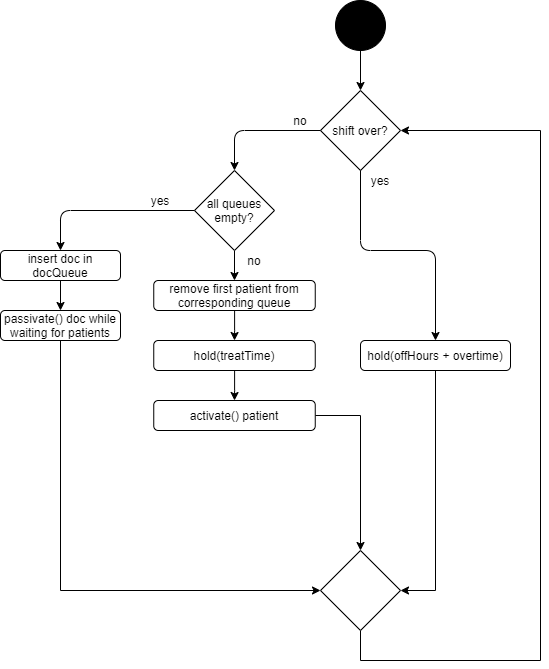
\includegraphics[width=\textwidth]{img/docProcess.png}
\textit{Vereinfachte Version des 'LifeCycle' des DocProcess}

\subsection{EmergencyModel}
\begin{itemize}
    \item TODO
    \item In dieser Klasse befinden sich die \textit{main-method} und die Initialisierungsmethoden, sowie jene die zur Darstellung der Werte mit JFree benötigt werden
\end{itemize}

\subsection{Erweiterung: Stoßzeiten}
... TODO

\subsection{Erweiterung: Todesfälle}
... TODO

\section{Simulationsergebnisse}
\subsection{Durchschnittliche Werte nach 50 runs (ca. 720 patients)}
Es wurden 50 Durchläufe zu je 22 Tagen (2 Tage Initialisierungsphase + 20 Tage Beobachtungszeitraum) gewählt, um Aussagekräftige Werte zu erhalten.\\
\begin{center}
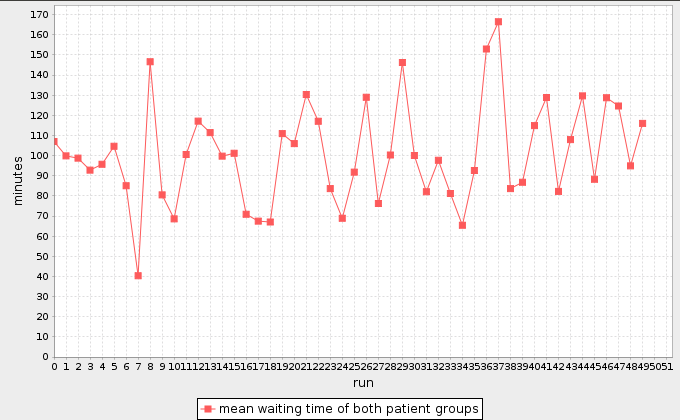
\includegraphics[scale=0.35]{img/avg_waiting.png}\\
\textit{Durchschnittliche Wartezeit bei allen Patientengruppen}\\
\end{center}
Wie schon anhand der Durschnittlichen Wartezeiten absehbar, sind diese teilweise sehr unterschiedlich bei den verschiedenen Durchgängen (also im Wertebereich zwischen ca. 40 und 170 Minuten).
.\\
\begin{center}
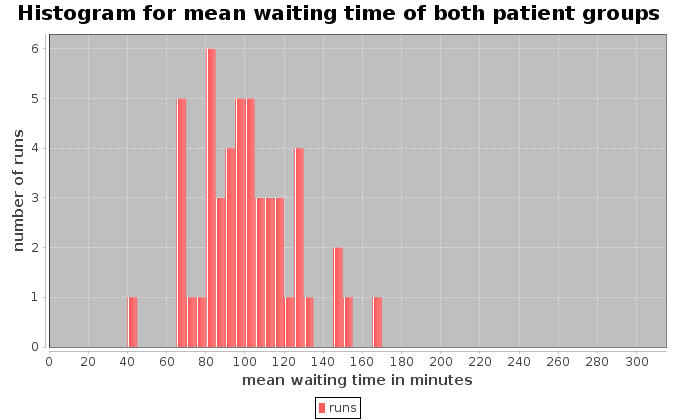
\includegraphics[scale=0.4]{img/avg_wait_histogram.png}\\
\textit{Histogramm: Durchschnittliche Wartezeit bei allen Patientengruppen}\\
\end{center}
Anhand des Histogramms zu diesen Durschnittswartezeiten sieht man aber die ungefähre Normalverteilung dieser Werte, weshalb hiermit schon Aussagen getroffen werden können.
.\\
\begin{center}
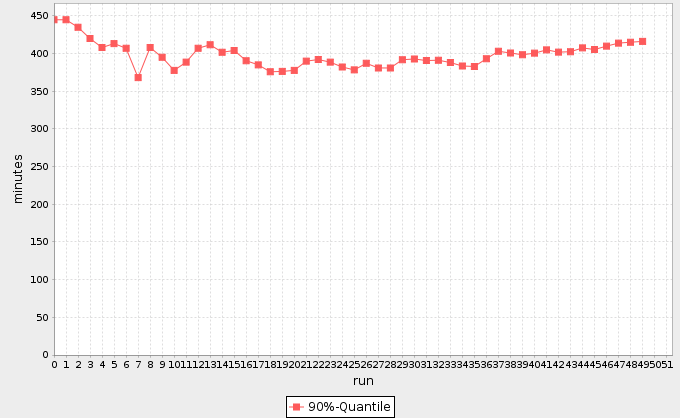
\includegraphics[scale=0.4]{img/quantile.png}\\
\textit{90\% Quantile}\\
\end{center}
Die 90\% Quantile soll hier die gesamte Aufenthaltsdauer in der Notaufnahme wiederspiegeln und erreicht ihr Maximum bei den 50 Durchläufen bei ca. 450 Minuten was in etwa 7.5 Stunden entspricht. Dieser Wert scheint durchaus realistisch.
.\\
\begin{center}
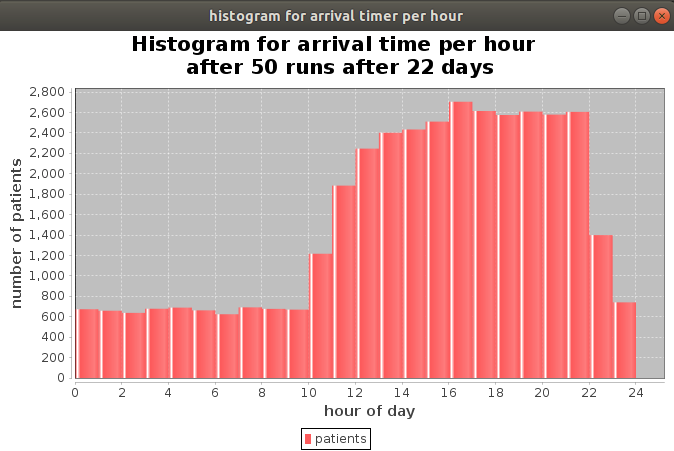
\includegraphics[scale=0.4]{img/day_night.png}\\
\textit{Ankunftszeit der Patienten über den Tag, um des Tag/Nacht Zyklus ersichtlich zu machen}
\end{center}
.\\
\begin{center}
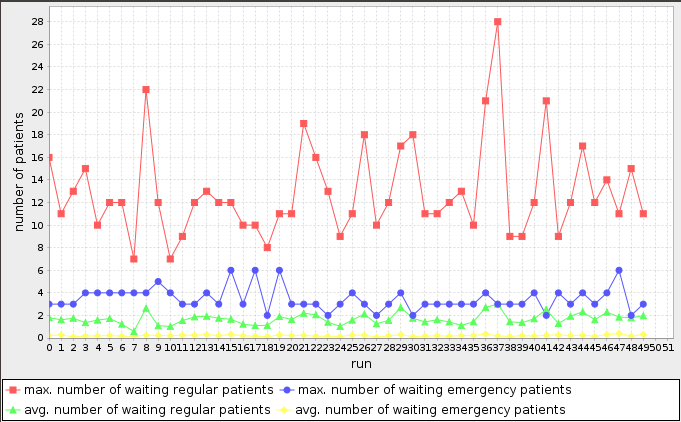
\includegraphics[scale=0.4]{img/max_avg_patients.png}\\
\textit{Maximale und durchschnittliche Wartezeit jeweils der Notfallpatienten und der regulären Patienten}\\
\end{center}
Wichtig hier ist, dass die Maximale Anzahl an wartenden Notfallpatienten niemals die der regulär wartenden Patienten übersteigt. Was deutlich ersichtlich ist. Interessant allerdings auch, ist dass die maximale Anzahl an regulär und Notfall-Patienten nicht unbedingt abhängig voneinander scheint, sondern eher zufällig. Die Durschnittliche Anzahl der wartenden Notfallpatienten scheint sehr gering und übersteigt niemals den Wert 1.
.\\
\begin{center}
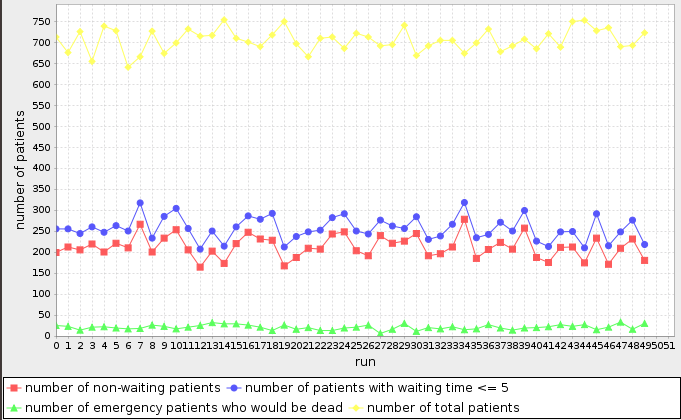
\includegraphics[scale=0.4]{img/not_less_waiting.png}\\
\textit{Anzahl der nicht-wartenden Patienten zusammen mit denen die weniger als 5 Minuten warten müssen, Anzahl der Patienten die in der Warteschlange verstorben wären und gesamte Anzahl der Patienten}\\
\end{center}
Verglichen mit der totalen Anzahl an Patienten ist die Anzahl derer die gar nicht oder weniger als 5 Minuten warten müssen nicht so schlecht. Also Anteil wäre hier ca. 30\% bei Patienten die weniger als 5 Minuten warten müssen und ca. 25\% die Patienten die gar nicht warten müssen. Hier wird die gesamte Wartezeit herangezogen, also es werden die Wartezeiten von Erst- und Zweitbehandlung aufsummiert. \\
.\\

\begin{tabular}{|l|l|}
\hline
\textbf{average of...} & \textbf{values}\\ \hline
max. number of waiting regular patients & 12.92 patients  \\ \hline
max. number of waiting emergency patients & 3.46 patients  \\ \hline
avg. number of waiting regular patients & 1.69 patients  \\ \hline
avg. number of waiting emergency patients & 0.21 patients  \\ \hline
mean waiting time of both patient groups & 100.80 minutes  \\ \hline
number of non-waiting patients & 212.22 patients  \\ \hline
number of patients with waiting time <= 5 & 255.82 patients  \\ \hline
90\%-Quantile & 397.99 minutes  \\ \hline
number of emergency patients who would be dead & 20.84 patients  \\ \hline
number of covid patients & 37.26 patients  \\ \hline
max number of waiting covid patients & 1.12 patients  \\ \hline
\end{tabular}\\
\begin{center}
\textit{Duchschnittliche Werte nach 50 runs}\\
\end{center}
Über alle Durchläufe gesprochen scheinen die Werte verglichen zu einer Notaufnahme relativ gut. Die Maximale Anzahl an wartenden regulären Patienten ist mit ca. 13 Patienten nicht schlecht. Wobei die Anzahl der wartenden Notfallpatienten mi 4 Patienten durch Erhöhung der Ärzteanzahl vielleicht verbessert werden sollte. Wäre hier eine Umsetzung auf eine reale Notfallaufnahme geplant. Auch die Anzahl der möglichen Todesfälle würde mit ca. 21 Patienten bestätigen, dass hier noch dringend mehr Ärzte eingestellt werden müssten. \\
Allerdings würde die Behandlung der potentiellen COVID Verdachtsfälle passen. Hier befindet sich kaum mehr als 1 Patient in der Warteschlange. Dh. die Gefahr, dass eine mit COVID Infizierte Person eine nicht infizierte Verdachtsperson ansteckt, ist sehr gering.

\end{document}

